\documentclass[11pt,a4paper]{article}
\usepackage[margin=2.3cm]{geometry}
\usepackage{graphicx}
\usepackage{booktabs}
\usepackage{amsmath}
\usepackage{xcolor}
\usepackage{tikz}
\usetikzlibrary{arrows.meta,positioning,decorations.pathmorphing,calc}
\usepackage[colorlinks=true,linkcolor=blue!50!black,urlcolor=blue!50!black]{hyperref}
\usepackage{caption}
\captionsetup{font=small,labelfont=bf}
\graphicspath{{figs/}}

\definecolor{verd}{HTML}{1a9850}
\definecolor{crim}{HTML}{c0392b}
\definecolor{blu}{HTML}{1f77b4}
\newcommand{\um}{\,\mu\mathrm{m/ns}}

\title{\textbf{The waveform-first forward-fit reconstruction\\ for the MX17 micro-TPC}\\
\large from ``why doesn't the track thread the reference?'' to a complete
reconstruction chain,\\ a resolved drift-velocity puzzle, a Magboltz-matched gas,
and in-situ drift-gap maps}
\author{MX17 June cosmic-bench analysis --- detectors A (det3), B (det2), E (det4)\\
\small primary dataset: det3 Saturday long run, resist 490\,V / drift 1000\,V,
M3 recipe $\chi^2<1$, NClus$=$4}
\date{25--27 July 2026}

\begin{document}
\maketitle

\begin{abstract}
\noindent
We rebuilt the micro-TPC reconstruction from the raw waveforms with no inherited
assumptions, to understand why reconstructed charge clusters did not ``thread''
the M3 reference track through the drift gap. The cause is a general property of
resistive-strip readouts: \emph{every} per-strip time estimate is extracted from
an aggregate waveform that mixes the strip's own charge with delayed, dispersed
copies of its neighbours' charge, compressing the time--position ladder by
20--30\% and making tracks look $\sim$40--50\% too steep. The fix is a
\emph{forward model}: fit the full waveform matrix with a track line, a
non-negative charge-depth profile, a measured pulse template and a calibrated
sharing kernel. On identical events this reaches a per-event angular residual of
$\sigma=1.0$--$1.1^\circ$ versus M3 (production ladder: $5$--$6^\circ$; previous
best hybrid: $1.5$--$1.6^\circ$), threads $\sim$70\% of tracks to $<1$\,mm over
the full gap, and a toy closure shows the remaining $\sim$$1^\circ$ is the
diffusion/charge-granularity \emph{physics floor} --- electronics noise
contributes only $0.02^\circ$. The method resolves the long-standing
drift-velocity tension ($v = 36.7\pm0.3\pm0.9\um$ at 1000\,V; the geometric
34.3 was biased by its spatial-floor subtraction), matches Magboltz for
Ar/iC$_4$H$_{10}$ 95/5 $+\,0.8\%$\,H$_2$O across the full drift scan, and turns
the deconvolved charge-arrival profile into an \emph{in-situ drift-gap map}:
det3's cathode plane is tilted by $\sim$2.7\,mm, det4's is bowed by
$\pm$3\,mm, and det2's is flat at the full 30\,mm gap. The chain is packaged
as a per-detector calibration protocol plus a production fitter
(\texttt{wft\_reco.py}), validated on three chambers.
\end{abstract}

\tableofcontents

%======================================================================
\section{Introduction: the threading problem}
%======================================================================

The MX17 chambers are read out as \textbf{micro-TPCs}: a muon crossing the
$\sim$30\,mm drift gap leaves a line of ionization; the electrons drift to the
micromegas mesh at constant velocity, so \emph{arrival time encodes depth}.
Each strip therefore measures a point $(\text{position},\,\text{time})$, and a
straight muon should appear as a straight ``ladder'' in the position--time
plane (Fig.~\ref{fig:principle}).

It did not. With hit-level reconstruction, the fitted ladders were
systematically $\sim$4$^\circ$ steeper than the M3 reference telescope tracks:
in 3-D event displays the reference threads the charge cloud at the mesh and
fans away from it with depth
(\texttt{REFERENCE\_TRACK\_THREADING\_REPORT.md}). Alignment was ruled out
(mesh residuals centred to $<10\,\mu$m); hit-level ``unsharing''
(deconvolution) fixed the bias only on ensemble average while adding per-event
noise. The question this work started from: \emph{can any reconstruction make
a single muon thread the reference line through the whole gap?}

\begin{figure}[htb]
\centering
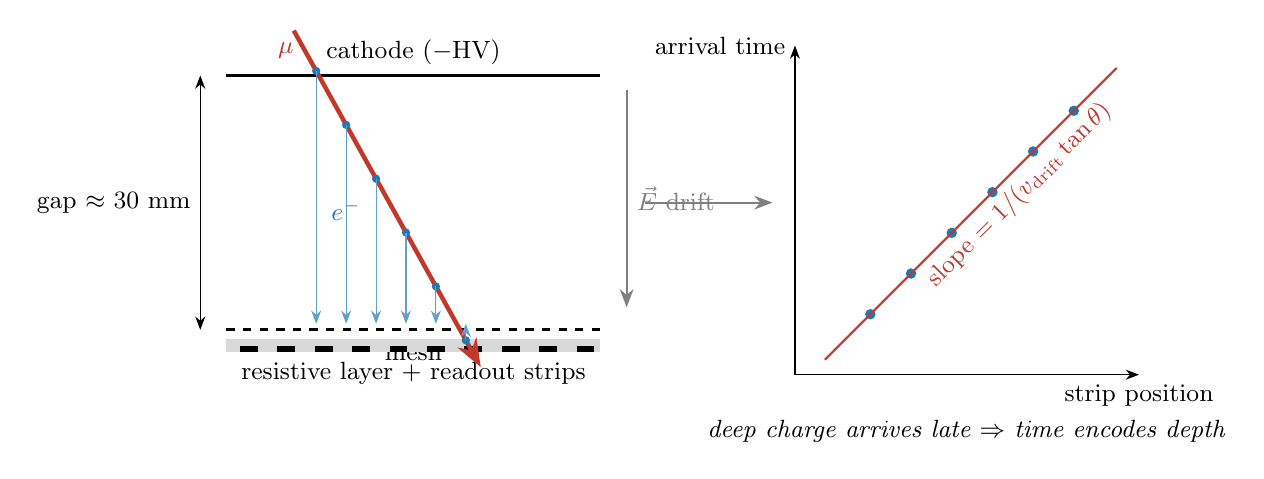
\begin{tikzpicture}[scale=0.95,>=Stealth]
% ---------- left: detector side view ----------
\begin{scope}
  % cathode and mesh
  \draw[very thick] (0,4.0) -- (5,4.0) node[midway,above]{\small cathode ($-$HV)};
  \draw[very thick,dashed] (0,0.6) -- (5,0.6) node[midway,below,yshift=-1pt]{\small mesh};
  \fill[gray!30] (0,0.30) rectangle (5,0.48);
  \node[below] at (2.5,0.30) {\small resistive layer + readout strips};
  \foreach \x in {0.3,0.8,...,4.8} \fill[black] (\x-0.12,0.30) rectangle (\x+0.12,0.38);
  % field arrow
  \draw[->,thick,gray] (5.35,3.8) -- (5.35,0.9) node[midway,right]{\small $\vec E$ drift};
  % muon track
  \draw[->,ultra thick,crim] (0.9,4.6) -- (3.4,0.1) node[pos=0.06,left]{\small $\mu$};
  % ionization electrons + drift lines
  \foreach \t in {0.12,0.28,0.44,0.60,0.76,0.92} {
    \pgfmathsetmacro{\px}{0.9+2.5*\t}
    \pgfmathsetmacro{\py}{4.6-4.5*\t}
    \fill[blu] (\px,\py) circle (0.055);
    \draw[->,blu!70,thin] (\px,\py) -- (\px,0.68);
  }
  \node[blu] at (1.6,2.2) {\small $e^-$};
  \draw[<->] (-0.35,0.6) -- (-0.35,4.0) node[midway,left]{\small gap $\approx$ 30 mm};
\end{scope}
% ---------- right: position-time ladder ----------
\begin{scope}[xshift=7.6cm]
  \draw[->] (0,0) -- (4.6,0) node[below]{\small strip position};
  \draw[->] (0,0) -- (0,4.4) node[left]{\small arrival time};
  \foreach \t in {0.12,0.28,0.44,0.60,0.76,0.92} {
    \pgfmathsetmacro{\px}{0.6+3.4*\t}
    \pgfmathsetmacro{\py}{0.4+3.4*\t}
    \fill[blu] (\px,\py) circle (0.07);
  }
  \draw[crim,thick] (0.4,0.2) -- (4.3,4.1);
  \node[crim,rotate=45] at (3.0,2.4) {\small slope $=1/(v_\mathrm{drift}\tan\theta)$};
  \node at (2.3,-0.75) {\small \emph{deep charge arrives late $\Rightarrow$ time encodes depth}};
\end{scope}
% connector
\draw[->,thick,gray] (5.6,2.3) -- (7.3,2.3);
\end{tikzpicture}
\caption{\textbf{The micro-TPC principle.} Left: a muon ionizes along its path;
electrons drift at constant $v_\mathrm{drift}$ to the mesh, are amplified, and
induce signals on the strips below. Right: each strip's charge-arrival time maps
its depth, so a straight track is a straight line in the position--time plane.
The reconstruction's job is to measure that line.}
\label{fig:principle}
\end{figure}

\begin{figure}[htb]
\centering
\includegraphics[width=0.98\textwidth]{event_raw.png}
\caption{\textbf{What the raw data looks like.} One cosmic muon in the det3
waveform matrix (colour = pedestal/common-noise-subtracted ADC, one column per
0.78\,mm strip, one row per 60\,ns sample). The inclined charge ridge is the
track; the dashed line is the M3 telescope prediction (drawn at
$v=36.6\um$). Note the $\sim$430\,ns trigger latency before the first charge
and the dark undershoot band after the pulses.}
\label{fig:raw}
\end{figure}

%======================================================================
\section{Why hit-based timing fails here: the sharing mixture}
%======================================================================

The resistive layer deliberately spreads each avalanche's signal to
neighbouring strips. The copy that a neighbour receives is \emph{delayed and
dispersed} (measured below: $\sim$29\% per first neighbour, delay
$\tau_s\!\approx\!47$\,ns, dispersion $\sigma_s\!\approx\!90$\,ns). Every strip
waveform is therefore a \emph{mixture} (Fig.~\ref{fig:mixing}): its own charge
at its own arrival time, plus neighbour charge at the neighbours' (different)
arrival times.

\begin{figure}[htb]
\centering
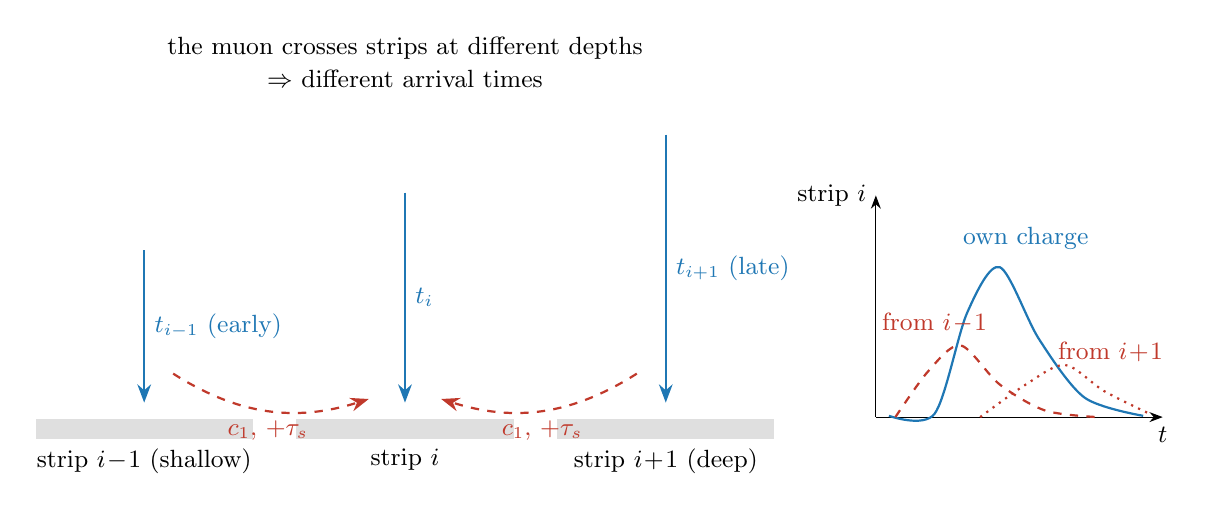
\begin{tikzpicture}[scale=0.92,>=Stealth]
% three strips
\foreach \i/\lab in {0/{strip $i\!-\!1$ (shallow)},1/{strip $i$},2/{strip $i\!+\!1$ (deep)}} {
  \fill[gray!25] (3.6*\i,0) rectangle (3.6*\i+3.0,0.28);
  \node[below] at (3.6*\i+1.5,0) {\small \lab};
}
% direct arrivals
\draw[->,thick,blu] (1.5,2.6) -- (1.5,0.5) node[midway,right]{\small $t_{i-1}$ (early)};
\draw[->,thick,blu] (5.1,3.4) -- (5.1,0.5) node[midway,right]{\small $t_i$};
\draw[->,thick,blu] (8.7,4.2) -- (8.7,0.5) node[midway,right]{\small $t_{i+1}$ (late)};
% sharing arrows into strip i
\draw[->,thick,crim,dashed] (1.9,0.9) to[bend right=25] node[below,midway]{\small $c_1$, $+\tau_s$} (4.6,0.55);
\draw[->,thick,crim,dashed] (8.3,0.9) to[bend left=25] node[below,midway]{\small $c_1$, $+\tau_s$} (5.6,0.55);
\node[align=center] at (5.1,5.2) {\small the muon crosses strips at different depths\\
\small $\Rightarrow$ different arrival times};
% waveform sketch
\begin{scope}[xshift=11.6cm,yshift=0.3cm,scale=0.9]
  \draw[->] (0,0) -- (4.4,0) node[below]{\small $t$};
  \draw[->] (0,0) -- (0,3.4) node[left]{\small strip $i$};
  \draw[blu,thick] plot[smooth] coordinates {(0.2,0.02)(0.9,0.05)(1.4,1.6)(1.9,2.3)(2.5,1.2)(3.2,0.3)(4.1,0.02)};
  \draw[crim,thick,dashed] plot[smooth] coordinates {(0.3,0.0)(0.8,0.7)(1.3,1.1)(1.9,0.5)(2.6,0.1)(3.4,0.0)};
  \draw[crim,thick,dotted] plot[smooth] coordinates {(1.6,0.0)(2.3,0.5)(2.9,0.8)(3.5,0.4)(4.2,0.05)};
  \node[blu] at (2.3,2.75) {\small own charge};
  \node[crim] at (0.9,1.45) {\small from $i\!-\!1$};
  \node[crim] at (3.6,1.0) {\small from $i\!+\!1$};
\end{scope}
\end{tikzpicture}
\caption{\textbf{The mixing problem.} Strip $i$'s waveform (right) is the sum of
its own charge (solid) and delayed, dispersed copies of both neighbours' charge
(dashed/dotted) --- which arrived at \emph{different} times because the track
crosses each strip at a different depth. Any single number extracted from this
aggregate (threshold, CFD, matched filter\ldots) is pulled toward the
cluster-mean time.}
\label{fig:mixing}
\end{figure}

The consequence is measured in Fig.~\ref{fig:scurve}: per-strip times (any
estimator) are too \emph{late} near the mesh end of the track and too
\emph{early} at the deep end --- an S-shaped compression of the ladder by
20--30\%. Read with the physical drift velocity, a compressed ladder is a track
that is too steep in space; this is the entire ``fans away with depth''
effect. Because the distortion lives in the aggregate waveform itself,
\emph{no better per-strip time estimator can fix it}. It must be modelled.

\begin{figure}[htb]
\centering
\includegraphics[width=0.9\textwidth]{estimator_residual_curves.png}
\caption{\textbf{Estimator-independent ladder compression.} Median per-strip
time residual versus the reference-implied arrival time (per-event $t_0$
floated), for two very different time estimators. Both are $\sim$$+40$\,ns late
at the mesh and $-100$\,ns early at the cathode.}
\label{fig:scurve}
\end{figure}

%======================================================================
\section{The forward model}
%======================================================================
\label{sec:model}

Instead of extracting times and fitting points, we \emph{predict the entire
waveform matrix} from a physical track hypothesis and fit the raw samples
(Fig.~\ref{fig:flow}). Sharing is applied \emph{forward} in the model --- never
inverted --- which is numerically well-conditioned where deconvolution is not.

\paragraph{Parameters (per plane).} A track line in position--time space,
\[
  \mathrm{pos}(u) = p_0 + w\,u ,\qquad
  w = v_\mathrm{drift}\tan\theta \;\;[\mathrm{mm/ns}],
\]
with $u$ the drift time since the mesh crossing at $t_0$; plus a
\textbf{non-negative charge profile} $q_k$ in $K$ bins of 60\,ns of arrival
time (the amount of ionization arriving in each depth slice --- left free
because ionization fluctuates). Note $v_\mathrm{drift}$ never enters the fit
itself: $w$ is measured in mm/ns directly.

\paragraph{Model.} The predicted waveform of strip $i$ at sample time $t$:
\[
 m_i(t) \;=\; \sum_k q_k \Big[\, F_{ik}\, h(t-t_0-u_k)
 \;+\; c_1 (F_{i-1,k}{+}F_{i+1,k})\, h_s(t-t_0-u_k-\tau_s)
 \;+\; c_2 (\ldots 2\tau_s) \Big]
\]
where $F_{ik}$ is the geometric fraction of bin-$k$ charge landing on strip
$i$ (track-segment length $\otimes$ Gaussian spread
$\sigma_p(u)=\sqrt{\sigma_{p0}^2+D_p^2 u}$), $h$ is the \emph{measured}
impulse-response template (Fig.~\ref{fig:template}), and $h_s$ is the same
template dispersed by $\sigma_s$ --- the resistive sharing kernel
$(c_1,c_2,\tau_s,\sigma_s)$.

\paragraph{Fitting.} For fixed $(p_0,w,t_0)$ the model is \emph{linear} in the
charges $q_k$, solved by non-negative least squares in milliseconds; the three
track parameters are found by a coarse grid plus a small simplex
(\texttt{forward\_model3.py}, $\sim$0.1\,s/plane, 800 events in 42\,s on 14
cores). Saturated samples are censored (one-sided penalty). Per-channel gains
(measured spread only 1.4\%) are divided out.

\begin{figure}[htb]
\centering
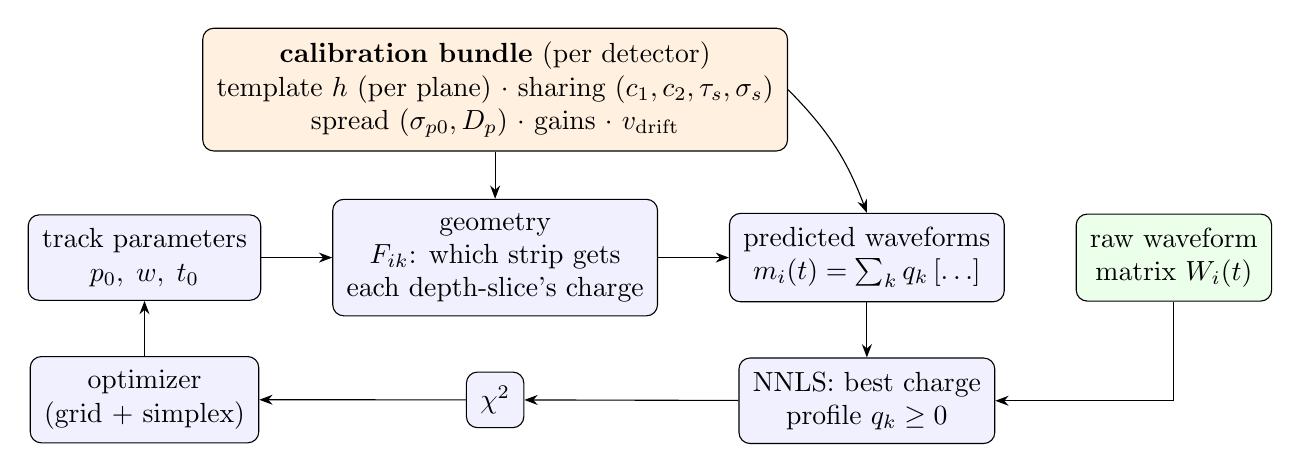
\begin{tikzpicture}[>=Stealth,node distance=5mm,
  box/.style={draw,rounded corners,align=center,fill=blue!6,inner sep=5pt},
  data/.style={draw,rounded corners,align=center,fill=green!8,inner sep=5pt},
  hyp/.style={draw,rounded corners,align=center,fill=orange!12,inner sep=5pt}]
\node[box] (par) {track parameters\\ $p_0,\; w,\; t_0$};
\node[box,right=9mm of par] (geo) {geometry\\ $F_{ik}$: which strip gets\\ each depth-slice's charge};
\node[hyp,above=6mm of geo] (cal) {\textbf{calibration bundle} (per detector)\\
template $h$ (per plane) $\cdot$ sharing $(c_1,c_2,\tau_s,\sigma_s)$\\
spread $(\sigma_{p0},D_p)$ $\cdot$ gains $\cdot$ $v_\mathrm{drift}$};
\node[box,right=9mm of geo] (mat) {predicted waveforms\\ $m_i(t)=\sum_k q_k\,[\ldots]$};
\node[data,right=9mm of mat] (dat) {raw waveform\\ matrix $W_i(t)$};
\node[box,below=7mm of mat] (nnls) {NNLS: best charge\\ profile $q_k \ge 0$};
\node[box,below=7mm of geo] (chi) {$\chi^2$};
\node[box,below=7mm of par] (opt) {optimizer\\ (grid + simplex)};
\draw[->] (par) -- (geo);
\draw[->] (geo) -- (mat);
\draw[->] (cal) -- (geo);
\draw[->] (cal.east) to[bend left=12] (mat.north);
\draw[->] (mat) -- (nnls);
\draw[->] (dat) |- (nnls);
\draw[->] (nnls) -- (chi);
\draw[->] (chi) -- (opt);
\draw[->] (opt) -- (par);
\end{tikzpicture}
\caption{\textbf{The fit loop.} The optimizer proposes a track line; the model
predicts every sample of every strip (charge profile solved linearly, with
positivity); the $\chi^2$ against the raw data drives the next proposal. Output:
track position, angle, charge-vs-depth profile, and honest per-event errors.}
\label{fig:flow}
\end{figure}

\begin{figure}[htb]
\centering
\includegraphics[width=0.72\textwidth]{templates_perplane.png}
\caption{\textbf{The measured impulse template} (median of $\sim$2000 bright
strips on steep tracks, where one strip's charge arrives nearly at once).
X and Y have identical rise (180\,ns 10--90) and width, but Y's undershoot is
4$\times$ deeper --- one reason the planes must be calibrated separately.}
\label{fig:template}
\end{figure}

\paragraph{Calibration protocol (per detector, automated).}
\begin{enumerate}\itemsep2pt
\item \textbf{Template}: median waveform of bright strips on steep tracks, per plane.
\item \textbf{Gain map}: per-channel data/model amplitude ratio (det3: 1.4\% spread).
\item \textbf{Hyper-fit}: with the track line \emph{pinned to the M3 reference}
on $\sim$150 medium-angle muons, fit
$(c_1,c_2,k_Y,\tau_s,\sigma_s,\sigma_{p0},D_p,v_\mathrm{drift})$ by minimizing
the summed waveform $\chi^2$. ($k_Y$ scales the Y-plane sharing.)
\end{enumerate}
det3 result: $c_1=0.29$, $c_2=0.05$, $k_Y=1.38$, $\tau_s=47$\,ns,
$\sigma_s=90$\,ns, $\sigma_{p0}=0.09$\,mm, $D_p=0.008$, $v=36.60\um$.
Anti-circularity controls: calibrating instead against the (biased) production
ladders converges 49\% \emph{worse} in $\chi^2$ with contorted parameters, and
free fits still pull toward the reference --- the waveforms genuinely prefer
the reference-sloped tracks.

\begin{figure}[htb]
\centering
\includegraphics[width=0.98\textwidth]{event_fit.png}
\caption{\textbf{One event, fitted.} Data, model, and normalized residual for
the X plane of the event in Fig.~\ref{fig:raw}. Fitted angle $10.9^\circ$ vs
M3 reference $10.4^\circ$.}
\label{fig:fit}
\end{figure}

%======================================================================
\section{Performance}
%======================================================================

\begin{figure}[htb]
\centering
\includegraphics[width=0.95\textwidth]{three_way_comparison.png}
\caption{\textbf{Head-to-head on identical events} (2{,}000-event disjoint test
set). Top: per-event angle residual vs M3. Bottom: cumulative worst deviation
of the fitted line from the reference line over the full 29\,mm depth.}
\label{fig:threeway}
\end{figure}

\begin{table}[htb]
\centering\small
\begin{tabular}{lcccc}
\toprule
reconstruction & angle $\sigma$ (x/y) & mesh $\sigma$ (x/y) & $<$1\,mm full depth & implied-$v$ flat?\\
\midrule
production raw ladder & $4.97^\circ/5.74^\circ$ & 0.67/0.76\,mm & 24\%/16\% & no (56$\to$39)\\
SOTA hybrid (unshared+cal.) & $1.58^\circ/1.53^\circ$ & --- & --- & ---\\
matched-filter ladder + remap & $1.51^\circ/1.86^\circ$ & 0.79/0.73\,mm & 54\%/52\% & no ($\pm$9)\\
\textbf{forward fit (v2)} & $\mathbf{1.06^\circ/1.10^\circ}$ & \textbf{0.57/0.59\,mm} & \textbf{74\%/70\%} & \textbf{yes} ($\pm$1)\\
\bottomrule
\end{tabular}
\caption{det3 benchmark, $|\tan\theta|\in[0.10,0.40]$, same events throughout.
The remap row is a cheap production pre-pass (matched-filter times + one trained
slope calibration): SOTA-level width but biased vs angle.}
\label{tab:bench}
\end{table}

Across \emph{all} angles the slope quality is flat at
$\sim$1.0--1.1$^\circ$ for $|\tan\theta|>0.04$ and degrades gracefully to
1.4$^\circ$(x)/2.4$^\circ$(y) below (timing carries no slope information on
1--2 strips; the production fitter flags these \texttt{slope\_reliable=False}
and can fall back to a joint two-plane fit). Mesh-position quality is
\emph{best} at near-vertical (0.47--0.53\,mm).

\paragraph{The physics floor.} A toy closure test (real geometries, real noise,
model-generated waveforms, known tracks) shows the fit recovers angles to
$\mathbf{0.02^\circ}$ with electronics noise alone; adding a 0.30\,mm RMS
transverse jitter to each 60\,ns depth-slice's charge centroid --- the expected
scale of transverse diffusion sampled by few avalanche-weighted electrons ---
reproduces the observed $1.05^\circ$ \emph{exactly}. \textbf{The residual
per-event scatter is detector physics, not reconstruction.} Component ablations
confirm robustness: no single model ingredient shifts the angle width by more
than $0.05^\circ$; the essential ingredients are the sharing kernel and the
per-plane template.

%======================================================================
\section{Drift velocity: the tension resolved, the gas identified}
%======================================================================

The calibration prefers $v=36.6\um$ while the previous geometric estimator gave
$34.3\um$. Four independent tests (Fig.~\ref{fig:vtension}) locate the
discrepancy entirely on the geometric side:
\begin{itemize}\itemsep2pt
\item the geometric method's \emph{time} ingredient (676\,ns) agrees with our
deconvolved gap-crossing duration (674\,ns); its \emph{extent column}
(23.2\,mm effective) disagrees with its own time-free measurement (24.5\,mm)
--- a 1.3\,mm ambiguity in subtracting the $\sim$2\,mm resistive-spread floor,
worth exactly the 5--7\% velocity difference;
\item toys calibrated with a deliberately wrong sharing truth at $v_\mathrm{true}=34$
return $33.1$: model mismatch \emph{deflates} $v$, it cannot inflate 34 into 36.6;
\item the profile likelihood (sharing re-fit at every $v$) has a sharp minimum
at 36.7 with weak $v\leftrightarrow$sharing degeneracy;
\item the fitted transverse speed divided by the reference tangent is flat vs
angle (physical), where the raw ladder's falls 56$\to$39 (unphysical).
\end{itemize}
\textbf{Result: } $v(1000\,\mathrm{V}) = 36.7 \pm 0.3\,(\mathrm{fit}) \pm
0.9\,(\mathrm{model})\um$.

\begin{figure}[htb]
\centering
\includegraphics[width=0.95\textwidth]{vtension_resolution.png}
\caption{\textbf{The velocity-tension resolution.} (a) profiled $\chi^2(v)$;
(b) the charge-visible column vs HV (see \S\ref{sec:gap} for the final
interpretation); (c) toy bias test; (d) the estimator family.}
\label{fig:vtension}
\end{figure}

Ref-pinned $\chi^2(v)$ scans on every drift-scan point give a smooth
$v(E)$ from 12 to 39$\um$ (300--1100\,V). Against a 71-mixture Magboltz
library (including 41 new tables computed this session, locally and on lxplus
condor, cross-validated to 0.01$\um$), the curve lands on
\textbf{Ar/iC$_4$H$_{10}$ 95/5 $+\,(0.81$--$0.86)\%$ H$_2$O} at RMS
0.63--0.67$\um$ for the operating fields (Fig.~\ref{fig:gas}) --- consistent
with the known bottle-drying trajectory that week. The 34-vs-36.6 question was,
in gas terms, a $\sim$0.5\% humidity ambiguity.

\begin{figure}[htb]
\centering
\includegraphics[width=0.63\textwidth]{v_vs_E_forward_refined.png}\hfill
\includegraphics[width=0.36\textwidth]{rms_vs_h2o.png}
\caption{\textbf{The gas.} Left: forward-fit $v(E)$ against the best Magboltz
mixtures. Right: RMS vs water fraction --- a clean parabola with minimum at
0.81--0.86\% H$_2$O. (The 300/500\,V measured points carry an extra
charge-basis caveat and should be re-scanned before quantitative reuse; the
$\ge$700\,V conclusion is unaffected.)}
\label{fig:gas}
\end{figure}

%======================================================================
\section{The drift-gap maps: an apparent 25\,mm gap that wasn't}
\label{sec:gap}
%======================================================================

The fitted charge profile $q_k$ is the template- and sharing-deconvolved
\emph{charge-arrival distribution}; for a through-going muon its endpoint
$U$ is the full-gap drift duration, so $v\cdot U$ measures the local gap.
A first pass gave an alarming $24.7$\,mm. Overnight adversarial review found
and fixed two estimator biases (a median over \emph{sparse} NNLS profiles, and
free-fit rather than reference-pinned profiles); the corrected, closure-validated
measurement is $U_{50}=762$\,ns $\Rightarrow$ \textbf{27.9\,mm}, stable against
the charge-basis length (Fig.~\ref{fig:kscan}), with toys recovering known
step-columns to $\le$5\,ns even under deliberate template mismatch.

Crucially, the data edge is \emph{soft} where toy step-gaps come back sharp:
the endpoint \textbf{varies with position}. Mapping $U_{50}$ versus the track's
location (Fig.~\ref{fig:gapmap}) shows det3's column running
26.5$\to$29.5\,mm --- a $\sim$2.7\,mm \textbf{tilt of the cathode plane along
y} plus a slight bow in x --- with a small additional electrostatic pull at
higher drift field (28.4$\to$27.8\,mm from 900$\to$1100\,V, the expected
$E^2$ trend). det4 shows its own $\pm$3\,mm bow (28.8\,mm average). The control:
\textbf{det2 (detector B) is flat at 30.5\,mm} --- the method reads the full
mechanical gap on a flat chamber.

\begin{figure}[htb]
\centering
\includegraphics[width=0.75\textwidth]{K_scan.png}
\caption{\textbf{Endpoint robustness.} The mean deconvolved charge profile at
1000\,V for charge-basis lengths $K=18\ldots30$: $U_{50}=762$\,ns for all
valid $K$ (junk accumulates only at $K=30$; closure toys quantify the regime).
Dotted/dashed guides: 25 and 29\,mm equivalents.}
\label{fig:kscan}
\end{figure}

\begin{figure}[htb]
\centering
\includegraphics[width=0.98\textwidth]{gap_map.png}
\caption{\textbf{det3's drift-gap topography}, measured in situ from cosmic
data alone: charge-column length vs track position. The y-tilt of
$\sim$2.7\,mm and slight x-bow are coherent across 7{,}240 profiles.}
\label{fig:gapmap}
\end{figure}

\begin{figure}[htb]
\centering
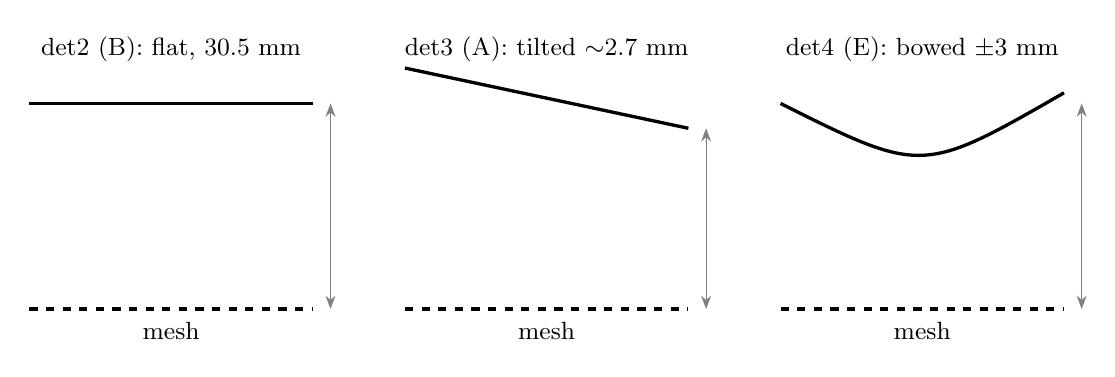
\begin{tikzpicture}[scale=0.9,>=Stealth]
\foreach \i/\name/\tilta/\tiltb in {0/{det2 (B): flat, 30.5 mm}/0/0,
                                    1/{det3 (A): tilted $\sim$2.7 mm}/0.5/-0.35,
                                    2/{det4 (E): bowed $\pm$3 mm}/0/0} {
 \begin{scope}[xshift=5.3cm*\i]
  \draw[very thick,dashed] (0,0) -- (4,0);
  \node[below] at (2,-0.05) {\small mesh};
  \ifnum\i=2
    \draw[very thick] (0,2.9) .. controls (2,1.9) .. (4,3.05);
  \else
    \draw[very thick] (0,2.9+\tilta) -- (4,2.9+\tiltb);
  \fi
  \node[above] at (2,3.35) {\small \name};
  \draw[<->,gray] (4.25,0) -- (4.25,2.9+\tiltb);
 \end{scope}
}
\end{tikzpicture}
\caption{\textbf{Chamber summary (cartoon).} The gap is nominal at the frame on
all three chambers; det3's cathode plane is tilted, det4's bowed, det2's flat.
Absolute scales carry each chamber's $v$ calibration ($\pm$3--5\%); the
patterns are robust.}
\label{fig:cartoon}
\end{figure}

Two corollaries: (i) gap-based velocity estimators inherited a $-3$ to $-7$\%
bias from assuming 29\,mm everywhere --- part of the historical velocity
confusion; (ii) the flat deconvolved profile shows the old amplitude-vs-depth
``attenuation'' is mostly diffusion + per-strip threshold, not charge loss.
The $U_{50}(x,y)$ map should simply become part of each chamber's calibration
bundle --- it is a free, in-situ flatness survey.

%======================================================================
\section{The production reconstruction stack}
%======================================================================

\begin{table}[htb]
\centering\small
\begin{tabular}{lcccc}
\toprule
 & det3 (A) & det2 (B) & det4 (E) \\
\midrule
kernel $c_1$ / $k_Y$ / $\tau_s$ / $\sigma_s$ & 0.29 / 1.38 / 47 / 90\,ns & 0.29 / 1.42 / 49 / 91\,ns & 0.24 / 2.36 / 68 / 234\,ns\\
$v_\mathrm{drift}$ (run conditions) & 36.6$\um$ & 39.9$\um$ & 34.2$\um$\\
angle $\sigma$ (x/y) & $1.06^\circ/1.10^\circ$ & $1.33^\circ/1.54^\circ$ & $2.00^\circ/1.97^\circ$\\
mesh $\sigma$ (x/y) & 0.57/0.59\,mm & 0.76/0.56\,mm & 0.93/0.71\,mm\\
column / topography & 27.9\,mm, y-tilt & 30.5\,mm, flat & 28.8\,mm, bowed\\
\bottomrule
\end{tabular}
\caption{The calibration protocol and fitter, run end-to-end on three chambers.
det2/det3 share a nearly identical sharing kernel (same production batch);
det4 is the gain-limited chamber and would profit from a refinement pass.}
\label{tab:fleet}
\end{table}

\noindent The deliverables, all in
\texttt{mx\_june\_cosmic\_qa/waveform\_first\_threading/}:
\begin{itemize}\itemsep2pt
\item \textbf{\texttt{wft\_reco.py}} --- production API. Loads a calibration
bundle; \texttt{fit\_plane()/fit\_event()} return position, angle, charge
profile, $\chi^2$, errors (statistical curvature $\oplus$ the $1^\circ$/0.33\,mm
physics floor), \texttt{slope\_reliable} and \texttt{quality\_ok} flags, and a
joint two-plane fallback for near-vertical planes.
\item \textbf{\texttt{forward\_model2/3.py}} --- the model and the fast fitter
($\sim$5$\times$ speedup, finds a lower $\chi^2$ than plain simplex in 20\% of
events; handles different DAQ window lengths).
\item \textbf{Calibration scripts} 03/11/12/13 (template, gains, hyper-fit) and
the per-chamber pipelines (26/26b/28/36).
\item \textbf{Physics tools}: ref-pinned $\chi^2(v)$ for gas monitoring
(works even at low HV where gap methods fail), the $U_{50}(x,y)$ gap mapper,
and the endpoint-closure toys that validate both.
\item A cheap \textbf{pre-pass} (matched-filter ladder + trained slope remap)
reaching SOTA-level width at negligible cost, for monitoring only.
\end{itemize}

%======================================================================
\section{Conclusions and next steps}
%======================================================================

The waveform-first forward fit turns the MX17 micro-TPC into what it was meant
to be: a per-event 3-D tracker with $\sim$1$^\circ$ angles and
$\sim$0.6\,mm positions, at the physical information limit set by diffusion
and charge granularity. Along the way it resolved the drift-velocity puzzle
($36.7\pm0.3\pm0.9\um$, gas = wet 95/5 at 0.8\% H$_2$O), retracted an apparent
short drift gap in favour of measured cathode-plane topography, and produced
per-chamber calibrations for three detectors.

\textbf{Open items:} (1) confirm the det3 tilt / det4 bow mechanically at the
next opening (no disassembly needed on this evidence alone); (2) an independent
humidity handle to pin $|v|$ below $\pm$1$\um$; (3) re-scan the 300/500\,V
velocities with the extended charge basis; (4) det4 refinement pass and the
remaining chambers (det6/7); (5) a numba/C++ port for another
$\sim$10$\times$ speed; (6) apply the chain to the July beam runs of the same
chambers.

\vfill
\noindent\small Reproduction: \texttt{WAVEFORM\_FIRST\_THREADING.md} \S8/\S15
and scripts 01--36 in the package directory. Figures and caches:
\texttt{<Analysis>/mx17\_3/waveform\_first/} (and \texttt{mx17\_2},
\texttt{mx17\_4} for detectors B/E).
\end{document}
